\documentclass[tikz,border=4pt]{standalone}
\usepackage{ctex}
\usepackage{amsmath}
\usetikzlibrary{arrows.meta}

% p8-02a: 一次函数四类图象（k>0, b>0） — 过一、二、三象限
\begin{document}
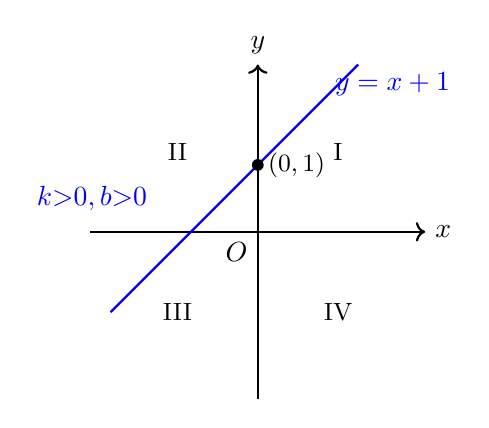
\begin{tikzpicture}[scale=0.85, thick]
  % 坐标轴
  \draw[->] (-2.5,0) -- (2.5,0) node[right] {$x$};
  \draw[->] (0,-2.5) -- (0,2.5) node[above] {$y$};
  \node[below left] at (0,0) {$O$};

  % k>0, b>0: y = x + 1
  \draw[blue, thick] (-2.2,-1.2) -- (1.5, 2.5);
  \fill (0,1) circle (2.5pt);
  \node[left, blue] at (-1.5, 0.5) {$k{>}0,b{>}0$};
  \node[right, blue] at (1.0, 2.2) {$y=x+1$};

  % 象限标注
  \node at (1.2,1.2) {\small I};
  \node at (-1.2,1.2) {\small II};
  \node at (-1.2,-1.2) {\small III};
  \node at (1.2,-1.2) {\small IV};

  % 纵截距标注
  \node[right] at (0,1) {\small$(0,1)$};

  % 虚线辅助
  \draw[gray, dashed] (-2.5,0) -- (-2.5,0);
\end{tikzpicture}
\end{document}
